\documentclass{beamer}

\mode<presentation> {

\usetheme{Copenhagen}
\usecolortheme{seagull}
}

\usepackage{graphicx}
\DeclareGraphicsExtensions{.pdf,.png,.jpg}
\usepackage{booktabs} % Allows the use of \toprule, \midrule and \bottomrule in tables
\usepackage{mathtools}
\usepackage{multirow}
\usepackage{color, colortbl}
\usepackage{minted}

%----------------------------------------------------------------------------------------
%	TITLE PAGE
%----------------------------------------------------------------------------------------

\title[Test]{Test}

\author{Rasmus Guldborg Pedersen}

\date{June 2015}

\begin{document}

\begin{frame}
\titlepage
\end{frame}

\begin{frame}
\frametitle{Overview}
\tableofcontents
\end{frame}



\section{Q 1.7: Project and Test management}

\subsection{Waterfall}
\begin{frame}
    \frametitle{Waterfall Model}
    \centering
    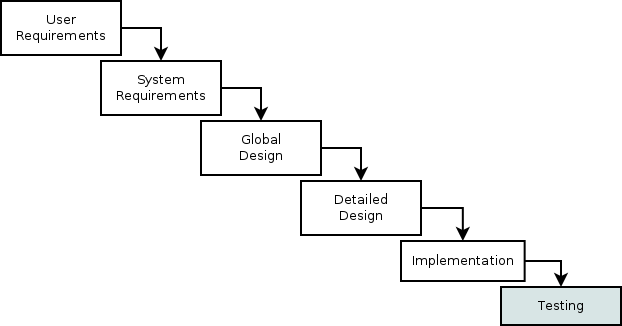
\includegraphics[scale=0.4]{waterfall.png}
    % Testing gets squeezed
    % There is no way to fix the defects found during testing
\end{frame}

\begin{frame}
    \frametitle{V Model}
    \centering
    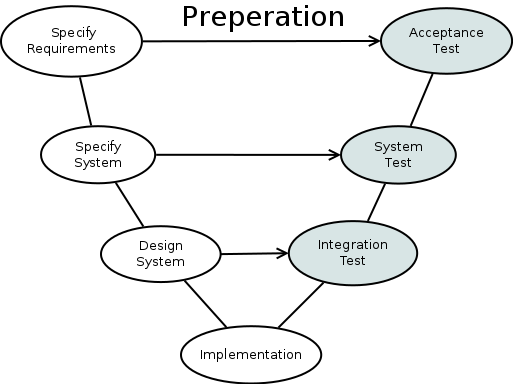
\includegraphics[scale=0.4]{v_model.png}
    % Testing starts earlier
\end{frame}

\begin{frame}
    \frametitle{W Model}
    \centering
    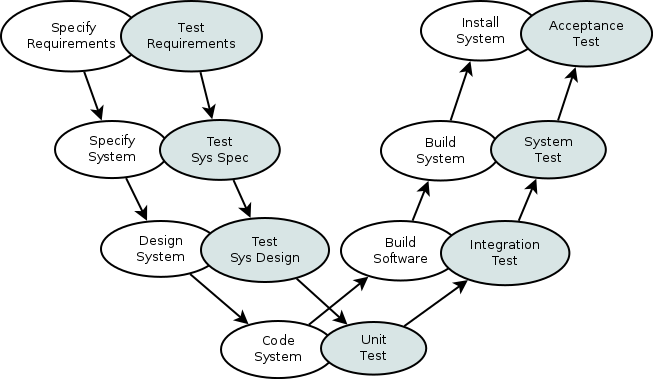
\includegraphics[scale=0.4]{w_model.png}
    % Testing is aligned with development
\end{frame}

\subsection{Agile}
\begin{frame}
    \frametitle{Scrum}
    \centering
    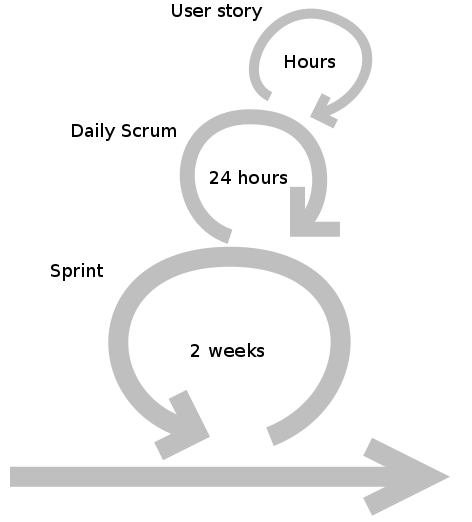
\includegraphics[scale=0.35]{scrum.png}
\end{frame}

\begin{frame}
    \frametitle{Agile Test Quadrants}
    \centering
    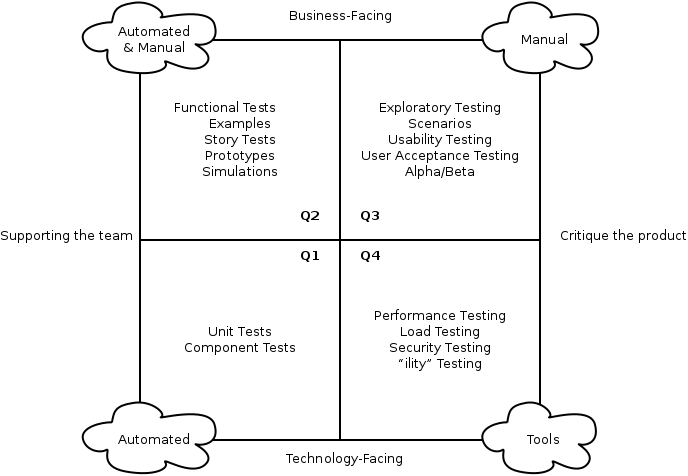
\includegraphics[scale=0.4]{agile_test_quadrants.png}
\end{frame}


%------------------------------------------------

\begin{frame}
    \frametitle{The End}

    %\Huge{\centerline{The End}}
    \begin{quote}
        ``Testing shows the presence, not the absence of bugs.''
        \raggedleft{--- Edsger W. Dijkstra}
    \end{quote}
\end{frame}

%----------------------------------------------------------------------------------------

\end{document}

